% Section 2: Introduction to Program Specifications
\section{Program Specifications}

\begin{frame}{What is a Program Specification?}
    \begin{block}{The Contract}
        A program specification acts as a formal contract. It precisely describes the expected behavior of a piece of code.
        \begin{itemize}
            \item It does \textbf{not} describe \emph{how} the program works.
            \item It \textbf{does} describe \emph{what} the program must accomplish.
        \end{itemize}
    \end{block}
    \begin{block}{Key Components}
        A specification consists of two main parts:
        \begin{itemize}
            \item \textbf{Precondition:} A condition that must be true \emph{before} the program is executed.
            \item \textbf{Postcondition:} A condition that is guaranteed to be true \emph{after} the program terminates.
        \end{itemize}
    \end{block}
\end{frame}

\begin{frame}{Visualizing a Specification}
    \framesubtitle{From Initial to Final State}
    \begin{center}
        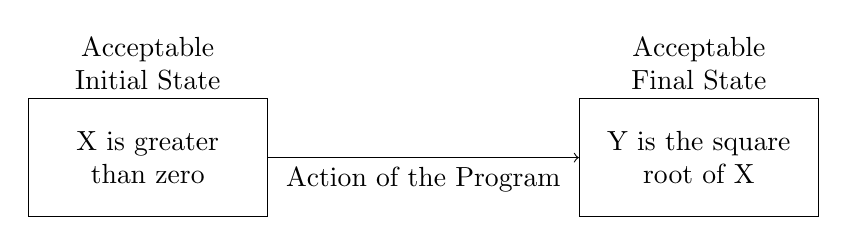
\begin{tikzpicture}
            % Define style for the boxes
            \tikzstyle{statebox} = [draw, rectangle, minimum height=1.5cm, text width=2.8cm, align=center]

            % Nodes for states
            \node [statebox] (initial) at (-1,0) {X is greater than zero};
            \node [statebox] (final) at (6,0) {Y is the square root of X};

            % Labels above the states
            \node [align=center] at (-1,1.2) {Acceptable \\ Initial State};
            \node [align=center] at (6,1.2) {Acceptable \\ Final State};

            % Arrow with label for the program's action
            \draw [->] (initial) -- node[below, align=center] {Action of the Program} (final);
        \end{tikzpicture}
    \end{center}
\end{frame}